\documentclass[12pt]{article}

\usepackage{graphicx} % for putting images
\usepackage{indentfirst} % for indenting the first line of a paragraph
\usepackage{hyperref}
\usepackage{xcolor}
\usepackage{subfig}
\usepackage{amsmath}
\usepackage{listings}
\usepackage{physics}
\usepackage{multirow}
\usepackage[nottoc,numbib]{tocbibind}


%New colors defined below
\definecolor{codeblue}{rgb}{0,0,0.6}
\definecolor{codegreen}{rgb}{0,0.6,0}
\definecolor{codegray}{rgb}{0.5,0.5,0.5}
\definecolor{codepurple}{rgb}{0.58,0,0.82}
\definecolor{backcolour}{rgb}{0.95,0.95,0.92}

%Code listing style named "mystyle"
\lstdefinestyle{mystyle}{
	backgroundcolor=\color{backcolour}, commentstyle=\color{codegreen},
	keywordstyle=\color{magenta},
	numberstyle=\tiny\color{codegray},
	stringstyle=\color{codepurple},
	basicstyle=\ttfamily\footnotesize,
	breakatwhitespace=false,		 
	breaklines=true,				 
	captionpos=b,					
	keepspaces=true,				 
	numbers=left,					
	numbersep=5pt,				  
	showspaces=false,				
	showstringspaces=false,
	showtabs=false,				  
	tabsize=2
}

\title{Quantum Robot}
\author{Aritra Mukhopadhyay}
\date{} % so that the date doesn't appear on top


% the next 5 lines help in removing the ugly
% boxes around links and making them look better
\hypersetup{
	colorlinks = true,
	urlcolor = black,
	linkcolor = black,
	citecolor = black,
}

\lstset{style=mystyle}
\begin{document}

	% The title of the document is placed here
	\begin{titlepage}
    \begin{center}
        \vspace*{1cm}

        \textbf{\Huge Quantum Robot}

        \vspace{1cm}
        {\Large Learning about Quantum Circuits Using Qiskit\\
        and about a basic Quantum Robot}
        \vfill

        
\includegraphics[width=6cm]{./images/IISER-K.png}
        
\includegraphics[width=6cm]{./images/NISER.jpg}
        \vfill

        \textbf{\large Prepared By:} Aritra Mukhopadhyay\\
        under the supervision of Prof.\ Prasanta K Panigrahi
        \vfill

        \today

    \end{center}
\end{titlepage}

	% adding the abstract
	\begin{abstract}
    Here is where I would say what is in this document.
\end{abstract}

	% adding the contents page
	\pagebreak
	\tableofcontents
	\addtocontents{toc}{~\hfill\textbf{Page}\par}


	
	% the different sections of the document
	\pagebreak
	\section{Introduction}

    The project primarily focused on learning and understanding quantum circuits. I thoroughly played around with IBM Quantum Experience and Qiskit to build intuitions about Quantum Gates and their uses in Quantum Circuits.

    I read some papers which were provided to me by Prof.\ Panigrahi. Soon I came across the paper~\cite{mahanti2019quantum}. While reading the paper, I came up with two easier solutions to the problem addressed in the paper. My report talks about those very solutions.  % introduction
	\section{Braitenberg Vehicles}

    Valentino Braitenberg (1926-2011) was an Italian neuroscientist and a synthetic psychologist. He spent most of his life doing experiments to understand how the animal nervous system works. He was also interested in building synthetic models of human or animal behaviour. He is well known for his book~\cite{braitenberg1986vehicles}. This book consists of a series of thought experiments about behaviours which can be expected of simple devices. All these thought experiments were inspired by animals and their nervous systems. He said ``when we analyse a mechanism, we tend to over-estimate its complexity".

    \subsection{Working of a Basic Braitenberg Vehicle}
    These are simple vehicles consisting of actively driven wheels and sensors. The sensors are stimulated by some stimulus (light, temperature, sound, presence of certain chemicals etc). The rotation speed of the wheels is directly controlled by the two sensor data. Depending upon how many sensors and wheels are there and how the sensor data influences the wheel speed (either excitatory or inhibitor), Braitenberg vehicles have been divided into the following categories:



    % Vehicle S1
    \subsubsection{Vehicle 1}
    \label{sec:Vehicle_1}

        \begin{figure}[t]%
            \centering
            \subfloat[\centering Excitatory Signal]{{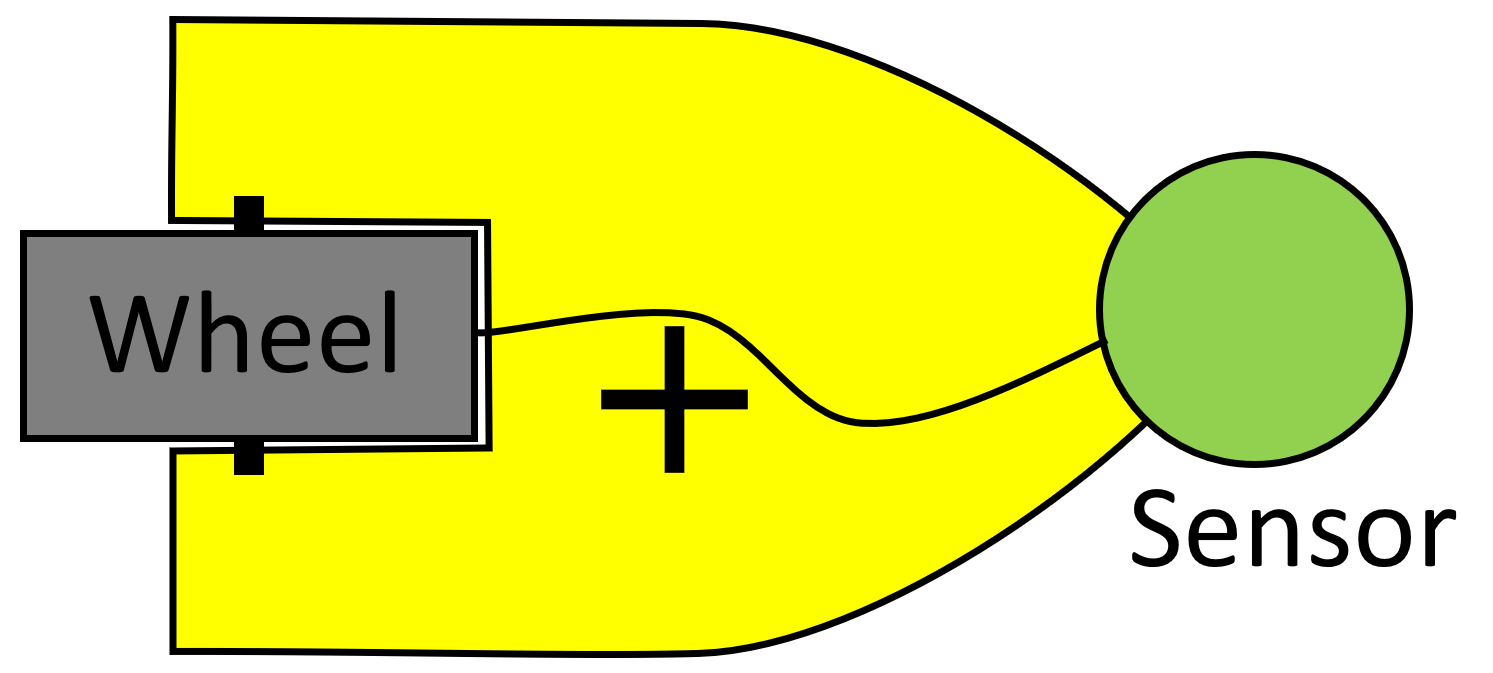
\includegraphics[width=5cm]{./images/1s_vehicle_p.png} }}%
            \qquad
            \subfloat[\centering Inhibitory Signal]{{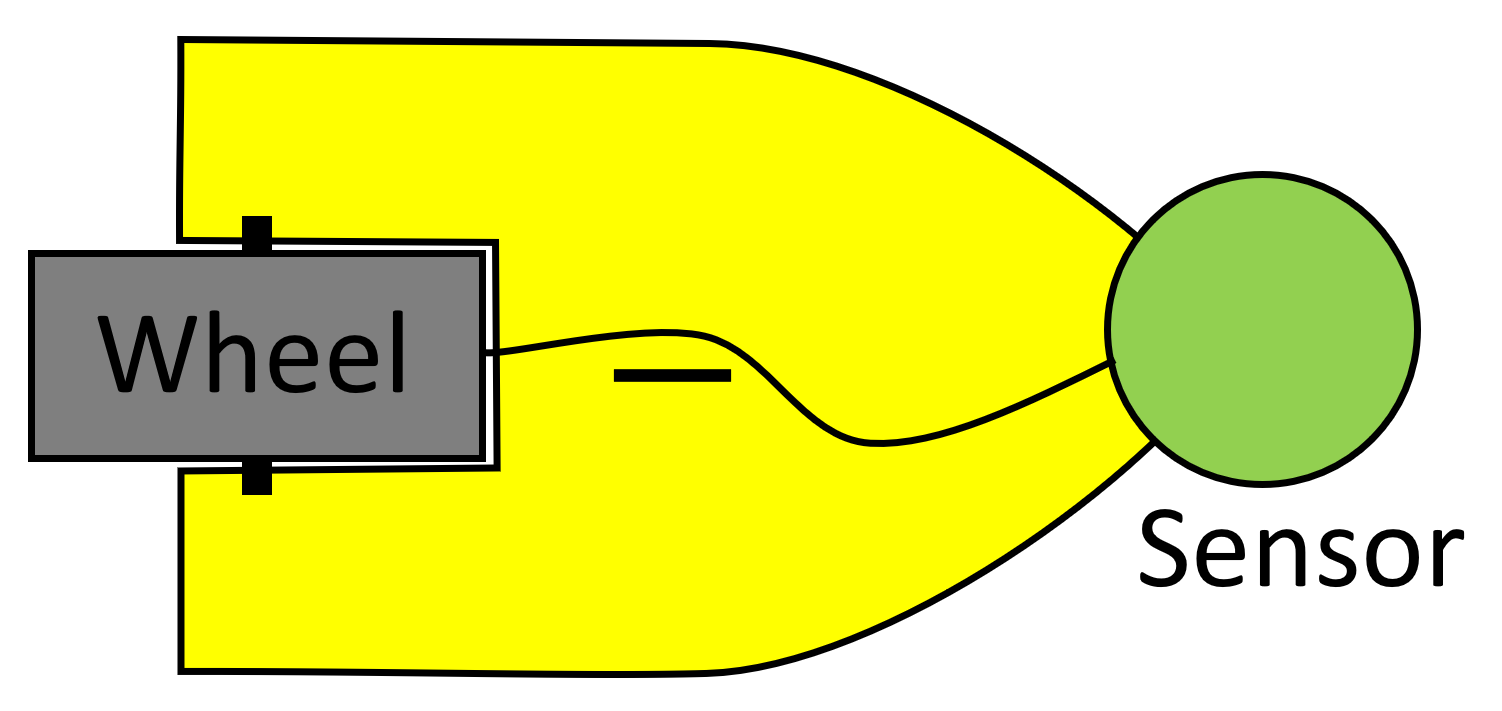
\includegraphics[width=5cm]{./images/1s_vehicle_m.png} }}%
            \caption{Braitenberg Vehicle Model 1}%
            \label{fig:vehicle1}%
        \end{figure}

        These vehicles (in Fig \ref{fig:vehicle1}) consist of a single sensor and a single wheel. These devices cannot change their directions. They move in a straight line. Now the sensor can either give an excitatory or an inhibitory signal to the wheel:

        \begin{itemize}
            \item \textbf{Excitatory Signal from Sensor:} Here, wheel speed is directly proportional to the strength of the stimulus. As the sensor senses more stimulus, (the stimulus is near) the wheel rotates faster; the vehicle gains speed. Thus, the speed of the vehicle is more when the vehicle is near the stimulus and the vehicle moves slowly when it is away from the stimulus. As a result, it spends less time near the source of stimulus and more time roaming away from it.
            \item \textbf{Inhibitory Signal from Sensor:} Here, wheel speed is inversely proportional to the strength of the stimulus. As the sensor senses more stimulus, the vehicle slows down. Thus, the devices gather around the source of stimulus.
        \end{itemize}


    % Vehicle S2
    \subsubsection{Vehicle 2}
    \label{sec:Vehicle_2}

        \begin{figure}[b]%
            \centering
            \subfloat[\centering Uncrossed Connection]{{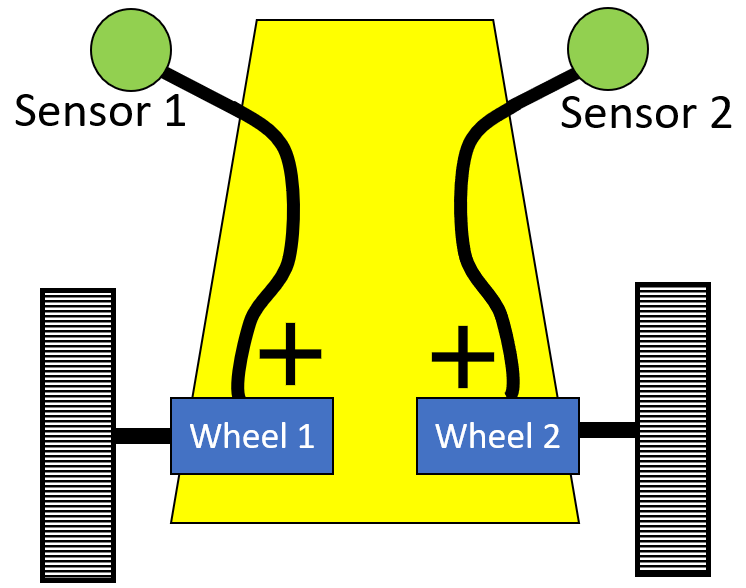
\includegraphics[width=5cm]{./images/2s_vehicle_d.png}}}%
            \qquad
            \subfloat[\centering Crossed Connection]{{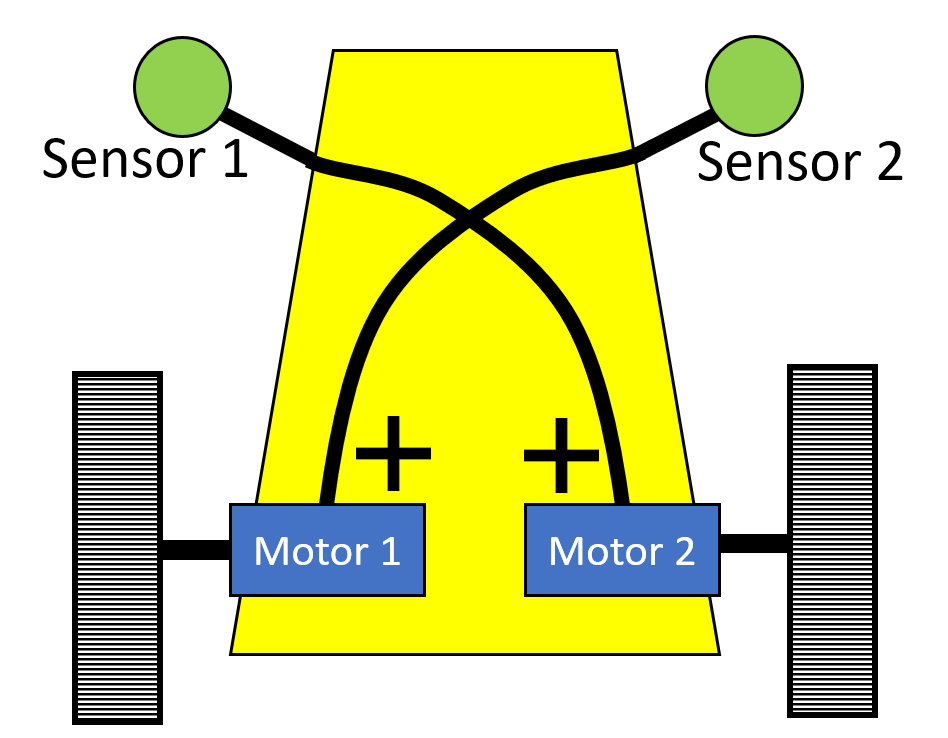
\includegraphics[width=5cm]{./images/2s_vehicle_c.png}}}%
            \caption{Braitenberg Vehicle Model 2}%
            \label{fig:vehicle2}%
        \end{figure}

        These vehicles (in Fig \ref{fig:vehicle2}) consist of two sensors and two wheels. Unlike \hyperref[sec:Vehicle_1]{Vehicle 1}, they can move freely on a 2D plane. But here, the sensors can always give an excitatory signal to the wheels. They have been divided into three categories depending upon their connections:

        \begin{itemize}
            \item \textbf{Uncrossed connections (2a):} Here, the left sensor is attached to the left wheel and the right sensor is attached to the right wheel. Now, suppose a source of stimulus is present on the right side of the vehicle, the right sensor is stimulated more than the left one. Hence the right wheel rotates faster than the left wheel. Thus the vehicle turns left and goes away from the stimulus.\\
            \textbf{Inference:} The vehicle expresses \textbf{fear} from the cause of the stimulus. And is termed as \textbf{`COWARD'} by Braitenberg.
            \item \textbf{Crossed connections (2b):} In this case, the left sensor is attached to the right wheel and the right sensor is attached to the left wheel. Now, to a stimulus on the right, the system responds by rotating the left wheel faster. It moves towards the stimulus. As it moves closer to the stimulus, its speed increases. Soon, the vehicle collides with the stimulus at great speed.\\
            \textbf{Inference:} The vehicle expresses \textbf{aggression/hate} towards the cause of the stimulus.
            \item \textbf{Double connections (2c):} Here, both the sensors are connected to both the wheels. As both the wheels symultaneously recieve the same signal, this vehicle cannot turn (turning is achieved by different speed of the wheels). Thus, despite having a more complex connection, the vehicle is inferior to both 2a and 2b vehicles.\\
            \textbf{Inference:} More complex connections do not always give us more complex functionality.
        \end{itemize}

        In general, all the types of Vehicle 2 dislike the presence of the stimulus in their vicinity.

    % Vehicle S3
    \subsubsection{Vehicle 3}
    \label{sec:Vehicle_3}

    \begin{figure}[b]%
        \centering
        \subfloat[\centering Uncrossed Connection]{{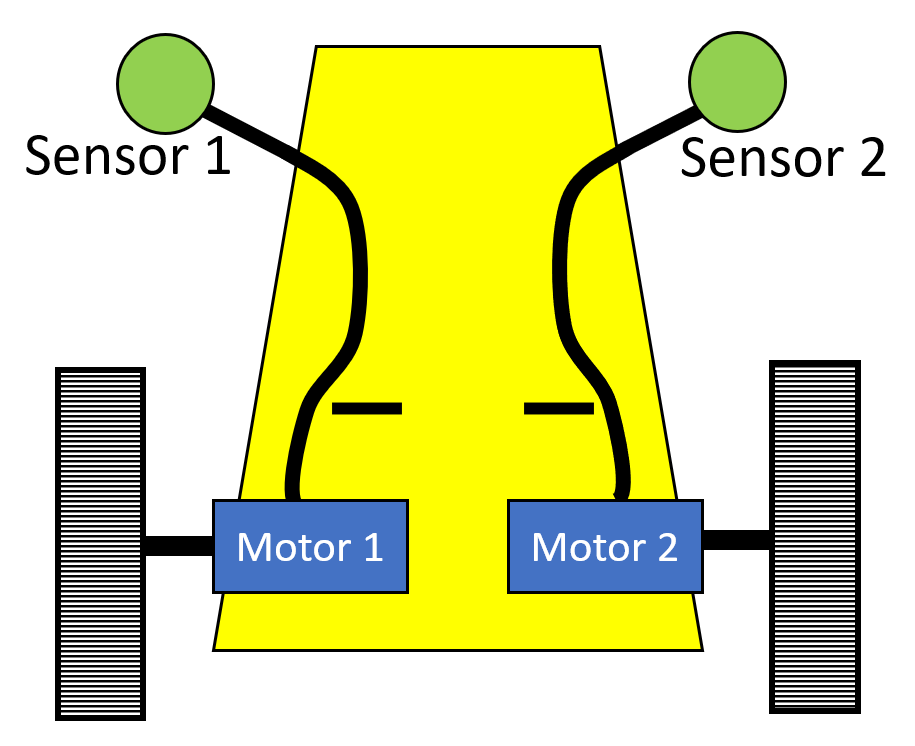
\includegraphics[width=5cm]{./images/3s_vehicle_d.png}}}%
        \qquad
        \subfloat[\centering Crossed Connection]{{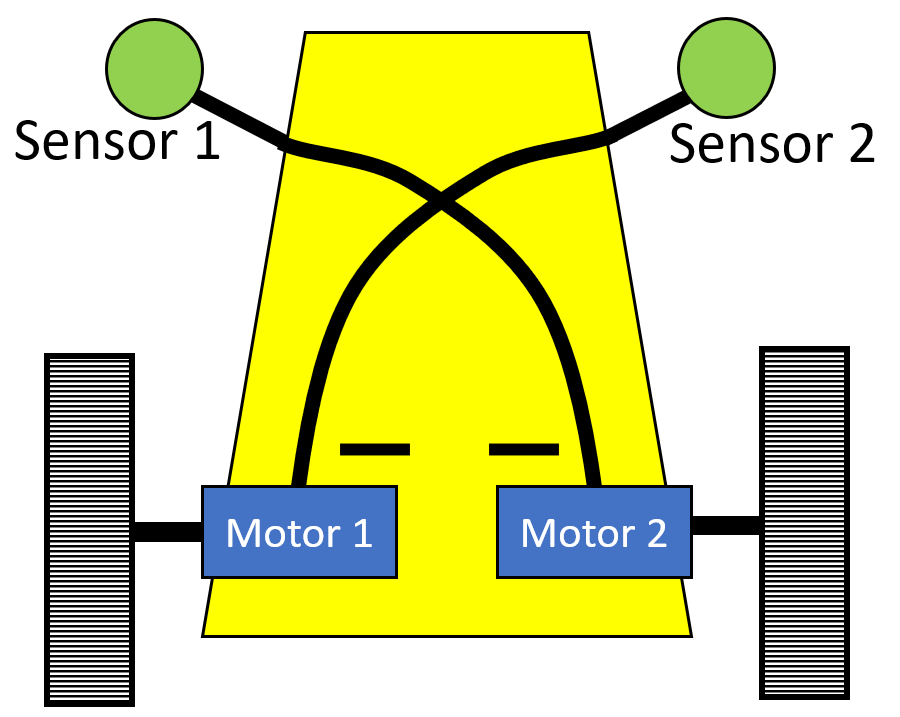
\includegraphics[width=5cm]{./images/3s_vehicle_c.png}}}%
        \caption{Braitenberg Vehicle Model 3}%
        \label{fig:vehicle3}%
    \end{figure}

    Just like the \hyperref[sec:Vehicle_2]{Vehicle 2} These vehicles (in Fig \ref{fig:vehicle3}) also have two sensors and two wheels. As a result, they also have full manoeuvring control over the plane (2D). But here, the sensors can always give an inhibitory signal to the wheels. In absence of a stimulus, the wheels rotate at full speed, and the speed decreases on detection of stimulus. Depending upon their connections, they are of 3 types:

    \begin{itemize}
        \item \textbf{Uncrossed connections (3a):} The sensors are connected to their respective wheels. A stimulus on the right side of the vehicle slows down the right wheel. Thus the vehicle turns right and turns toward the stimulus. After turning, it has the stimulus just in front of it. Hence, both the wheels slow down and move at the same speeds. The vehicle heads towards the stimulus. The strength of the stimulus increases. Speed of the vehicle decreases. Finally, it comes to a halt near the stimulus.\\
        \textbf{Inference:} The vehicle expresses \textbf{love} for the cause of the stimulus. It sticks to the first stimulus it sees in its life. It does not care about anything else, nor does it go to other, more powerful stimuli.
        \item \textbf{Crossed connections (3b):} The left wheel is slowed by the right sensor and the left sensor slows down the right wheel. In the presence of a stimulus, although it moves away from it, it slows down. It spends some time near the stimulus but eventually moves away in search of new, stimuli.\\
        \textbf{Inference:} Braitenberg describes this vehicle as an \textbf{explorer}.
    \end{itemize}

    Braitenberg talked about a lot of other sorts of vehicles. Some had different types of sensors attached to the same vehicle (maybe one pair of sensors detects temperature, another detects heat etc.) all of them give either positive or negative responses and may be connected in a crossed or uncrossed fashion. Some vehicles might have a different graph of influence (All this while we were talking about a proportional influence of sensors on wheels. But this might not always be the case. For example, an influence might be drastic, there is no slowing down - if the sensor receives a particular amount of stimulus, it completely turns the wheel on or off.). There are a lot of other types of simple vehicles discussed in detail by Braitenberg in his book. But this much discussion is enough for the purpose of this report.

  % britenberg vehicles
	% \documentclass[main.tex]{subfiles}

% The Problem and Modified Design
\section{The Problem and Modified Design}
    
    \subsection{The Problem}
    We know that the 2b vehicle discussed above crashes into the stimulus with great speed. It shows aggression. That is not a very desirable thing to happen. Our main goal is to fix that and come up with a solution using quantum phenomena. To achieve this we modify the vehicle a bit. Till now, our vehicle was moving on a 2D plane. To avoid the collision we tried to get help from the 3rd dimension.
    
    \subsection{Proposed Modified Design}
    We have seen that the \hyperref[sec:Vehicle_1]{Vehicle 1} has a single wheel and it only moves along a straight line (1 wheel can only give us 1-dimensional motion). As we add another wheel in \hyperref[sec:Vehicle_2]{Vehicle 2} we get full access over the plane (2D). So, it is clear that to enable another degree of freedom, we have to add another actuator of some kind to make our vehicle fly above the stimulus (acts as an obstacle here).

    Now, \textit{`flying'} in the real world is a problem in itself. So we won't go into the details of how the vehicle achieves this flying motion. For the scope of this report, we assume that we have done the required arrangements for the vehicle to fly. We say for simplicity that we have attached a propeller on top of the vehicle. It makes the vehicle fly, like a helicopter. Here, we won't discuss problems like the vehicle itself rotating in the opposite direction as a result of the reaction force of the rotating propellers. Let that be a problem for another day.

        \begin{figure}[t]%
            \centering
            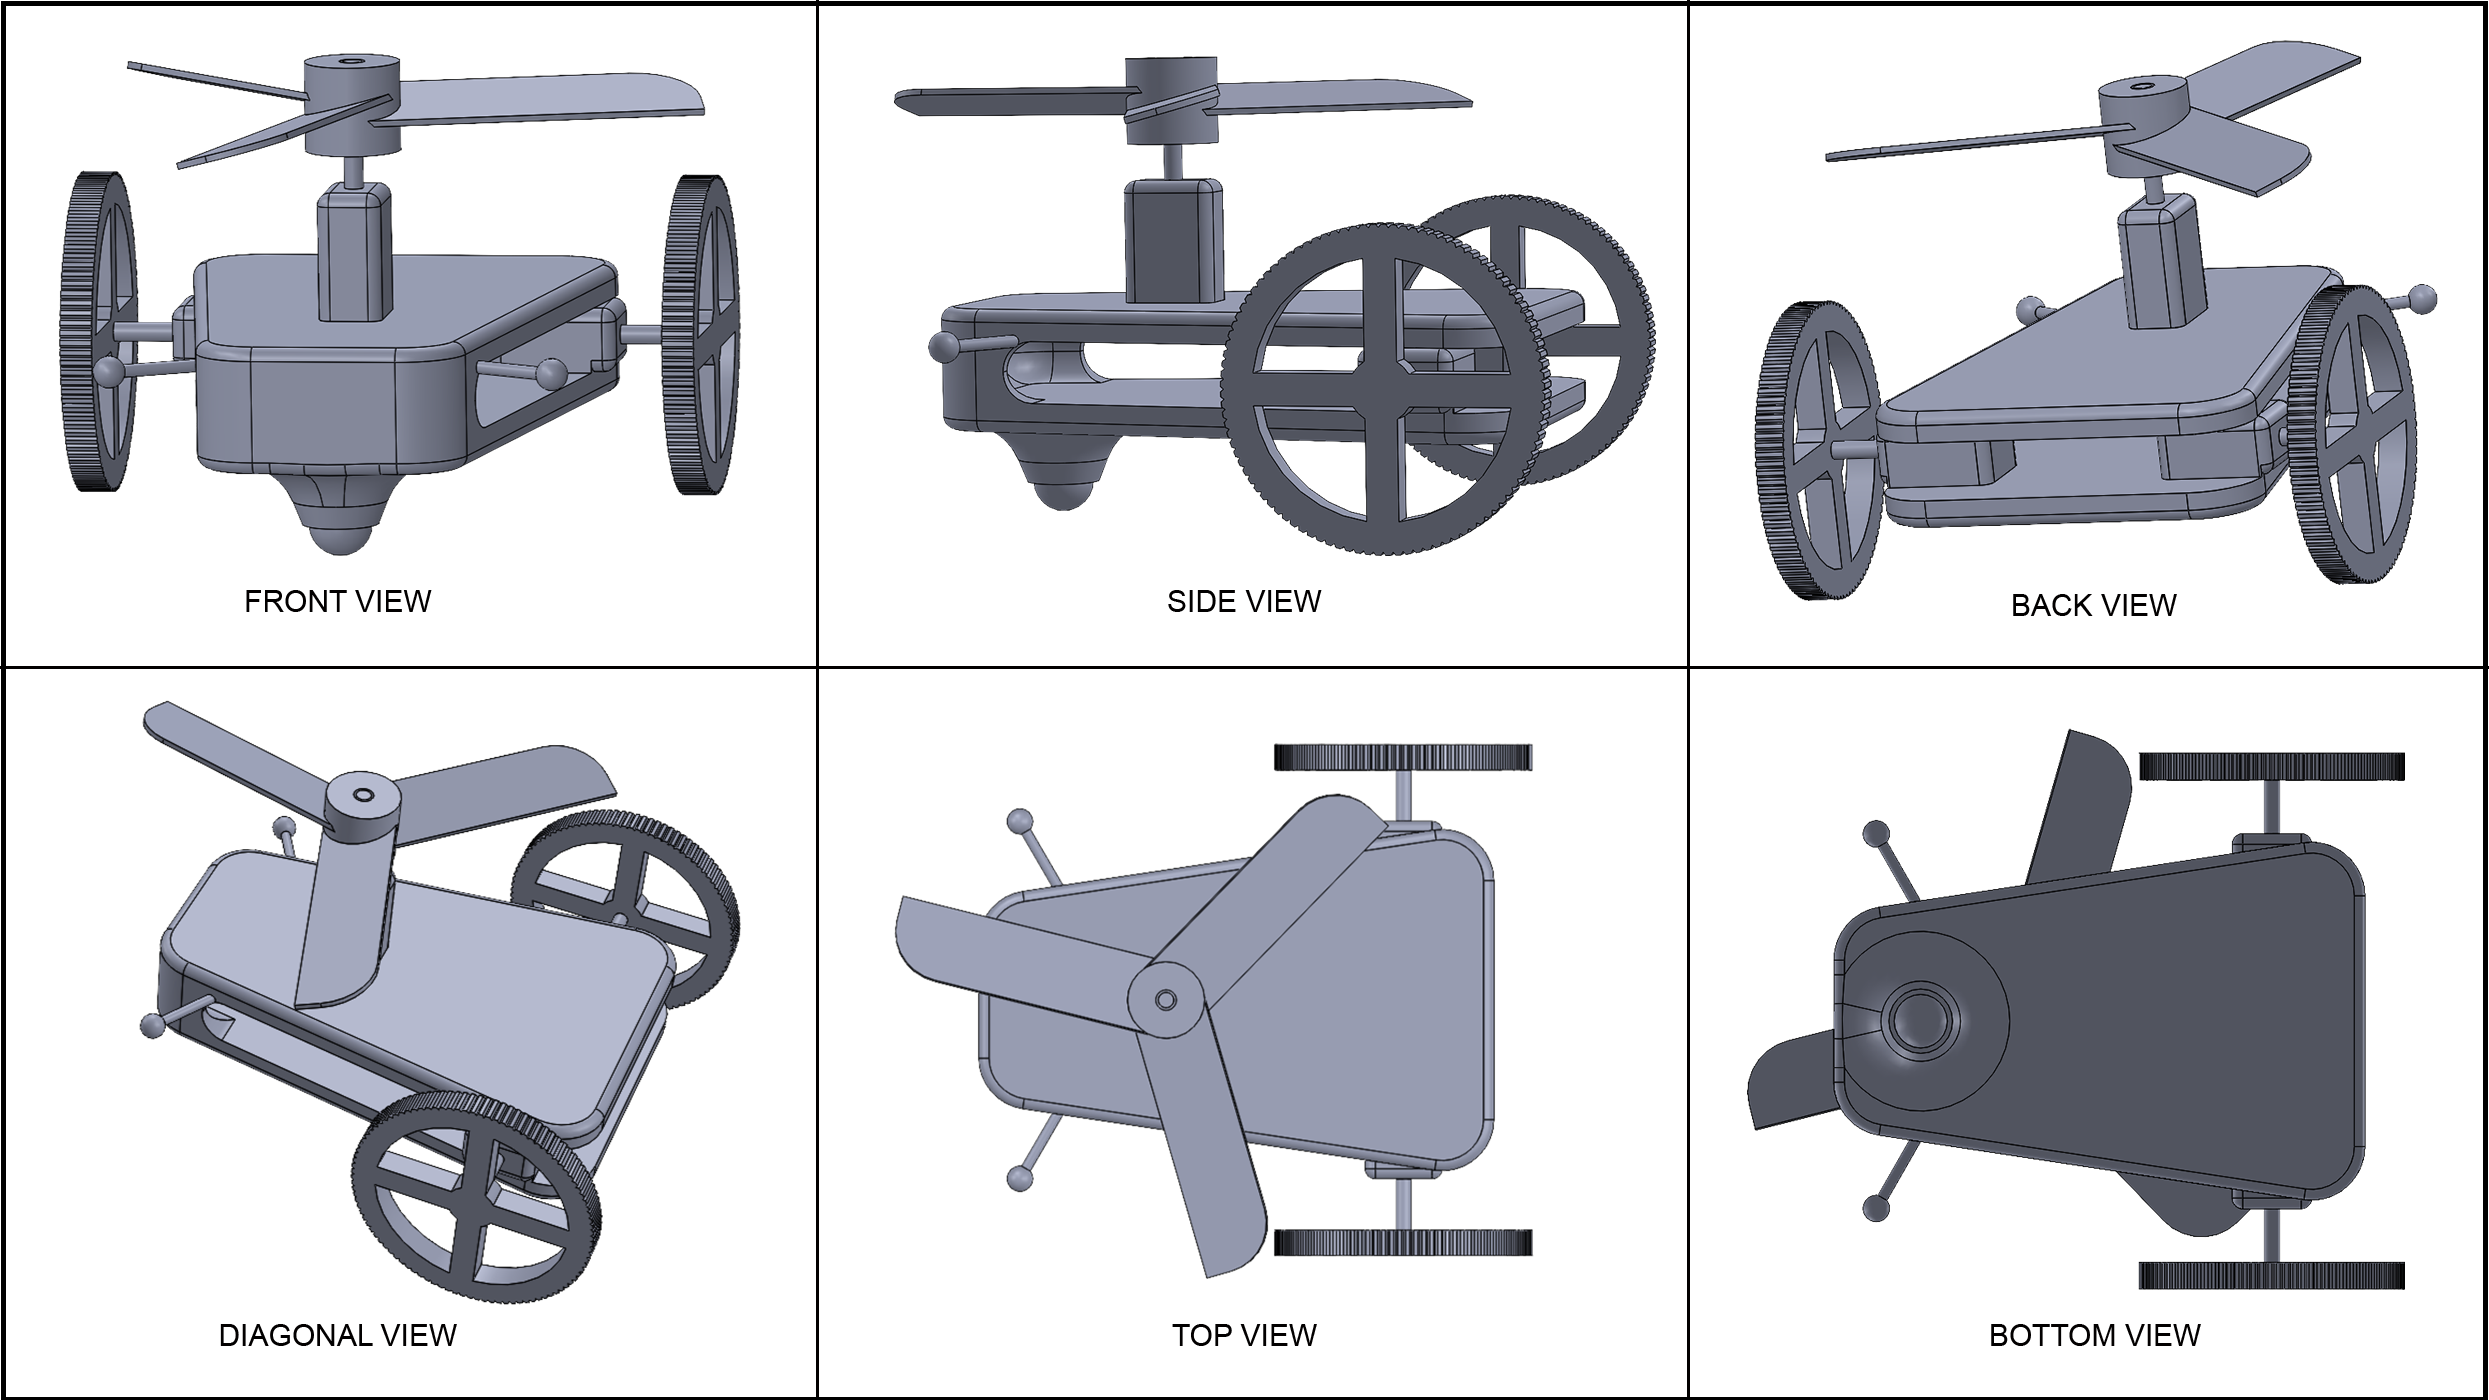
\includegraphics[width=14cm]{./images/vehicle_3D_grouped.png} 
            \caption{3D model of the proposed design}%
            \label{fig:3D_design}%
        \end{figure}

    So, finally, we are left with a vehicle which looks like Fig \ref{fig:3D_design}.
    \vspace{3mm}

    \subsection{Robot Configurations}
    \begin{itemize}
        \item \textbf{Sensors:} 2 sensors are attached on two sides of the vehicle for detecting the stimulus.
        \item \textbf{Actuators:} 2 wheels on two sides and 1 propeller on top for taking off the ground.
    \end{itemize}
% \end{document}
  % problem statement
	\section{Behaviour of the Vehicle}

Our vehicle behaves quite differently from any of the basic Braitenberg Vehicles. The vehicle is equipped with 2 quantum photosensors which return digital output ($\ket{0}$ or $\ket{1}$). Depending upon the sensor values, the wheels either rotate or do not rotate. When both the sensors give $\ket{0}$, both the wheels remain on. If one of the sensors is $\ket{1}$, the wheel of only that side remains on. If both the sensors are $\ket{1}$, and both the wheels are off, the propeller starts and the vehicle takes off. (the propeller remains off the rest of the time).


    \begin{table}[t]
        \centering
        \begin{tabular}{|cc|ccc|c|}
            \hline
            \multicolumn{2}{|c|}{\textbf{Sensor Output}}         & \multicolumn{3}{c|}{\textbf{Actuator Input}}                                                              & \multirow{2}{*}{\textbf{Behaviour}} \\ \cline{1-5}
            \multicolumn{1}{|c|}{\textbf{Left}} & \textbf{Right} & \multicolumn{1}{c|}{\textbf{Left Motor}} & \multicolumn{1}{c|}{\textbf{Right Motor}} & \textbf{Propeller} &                                     \\ \hline
            \multicolumn{1}{|c|}{0}             & 0              & \multicolumn{1}{c|}{1}                   & \multicolumn{1}{c|}{1}                    & 0                  & Moves Forward                       \\ \hline
            \multicolumn{1}{|c|}{0}             & 1              & \multicolumn{1}{c|}{0}                   & \multicolumn{1}{c|}{1}                    & 0                  & Turns Left                          \\ \hline
            \multicolumn{1}{|c|}{1}             & 0              & \multicolumn{1}{c|}{1}                   & \multicolumn{1}{c|}{0}                    & 0                  & Turns Right                         \\ \hline
            \multicolumn{1}{|c|}{1}             & 1              & \multicolumn{1}{c|}{0}                   & \multicolumn{1}{c|}{0}                    & 1                  & Takes off                           \\ \hline
        \end{tabular}
        \caption{Behaviour of the Vehicle}
        \label{table:1}
    \end{table}  % behaviour of the robot
	\section{My Solutions to the Problem}

	The car gets binary inputs ($\ket{0}$ and $\ket{1}$) from two sensors attached to it. We need to build a quantum circuit to give the output to the motors like the \hyperref[table:1]{\textit{Table 1}}.
	
	In the ~\cite{mahanti2019quantum} article, the authors tried to solve the problem by defining a new sort of quantum gate, the \textbf{two-control-two-target Toffoli (C\textsubscript{2}(X\textsuperscript{3}X\textsuperscript{4})) gate}. They also made a large Quantum Circuit. But, I found some much easier and smaller approaches to the problem.	
	\vspace{3mm}

	\noindent {\large From the \hyperref[table:1]{\textit{Table 1}}, we can say that:}
	
	\begin{itemize}
		\item M1 = not(S2) = $\sim$ S2
		\item M2 = not(S1) = $\sim$ S1
		\item M3 = S1 and S2 = S1 $\land$ S2
	\end{itemize}
	\noindent {\large I came up with two easier solutions:}
	\begin{enumerate}
		\item \textbf{5 cubit:} This approach uses 5 qubits. We use two Quantum Registers for the sensor inputs, and the rest three for the motor outputs.
		\item \textbf{3 cubit:} This approach uses 3 qubits. Here, we have two Quantum Registers for taking input from the two sensors. We process those signals and use them as inputs to the first two motor. We use the third Quantum Registers for output to the third motor.
	\end{enumerate}

	\subsection{Approach 1: 5 Cubit Solution}
	\label{solution:1}
		\subsubsection{Importing the libraries}
\label{code:importing_the_libraries}
\begin{lstlisting}[language=Python]
from qiskit import *
from qiskit.visualization import *\end{lstlisting}

\subsubsection{Making the Quantum Circuit}
\textbf{Making the Qiskit Classes:}
\label{code:making_the_qiskit_classes}
\begin{lstlisting}[language=Python]
# 1. making the sensor registers
sensors = QuantumRegister(2, 'sensor')
# 2. making the motor registers
motors = QuantumRegister(3, 'motor')
# 3. making the classical registers, 1 for each motors
creg_c = ClassicalRegister(3, 'measurements')
# 4. Adding the registers to get the quantum circuit
circuit = QuantumCircuit(sensors, motors, creg_c)\end{lstlisting}
\vspace{3mm}

\textbf{Initializing the Circuit:} Demonstrating initialization with sensor value as = $\ket{10}$. Please feel free to try out the other states ($\ket{00}$, $\ket{01}$ and $\ket{11}$). This is Similar to the digitalRead function of Arduino.
\label{code:initializing_the_circuit}
\begin{lstlisting}[language=Python]
ket_0 = [1, 0]
ket_1 = [0, 1]

# quantumRead = [ket_0, ket_0] # |00>
# quantumRead = [ket_0, ket_1] # |01>
quantumRead = [ket_1, ket_0]   # |10>
# quantumRead = [ket_1, ket_1] # |11>

circuit.initialize(quantumRead[0], [sensors[0]])
circuit.initialize(quantumRead[1], [sensors[1]])\end{lstlisting}
\vspace{3mm}

\textbf{Designing the circuit:}
\label{code:designing_the_circuit}
\begin{lstlisting}[language=Python]
circuit.ccx(sensors[0], sensors[1], motors[2])
circuit.x(sensors[0])
circuit.x(sensors[1])
circuit.cx(sensors[0], motors[1])
circuit.cx(sensors[1], motors[0])
circuit.barrier()
circuit.measure(motors[0], creg_c[2])
circuit.measure(motors[1], creg_c[1])
circuit.measure(motors[2], creg_c[0])
circuit.draw(output = 'mpl')\end{lstlisting}

\begin{figure}[h]%
	\centering
	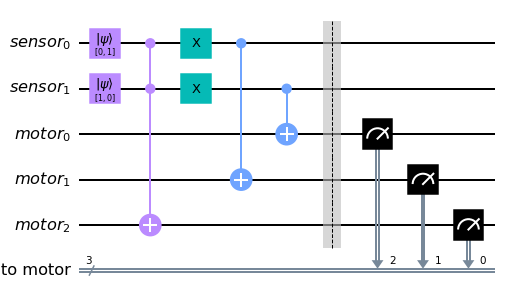
\includegraphics[width=0.9\linewidth]{./images/5qubit_qc.png}
	\caption{Circuit of the 5 Qubit Design}%
	\label{fig:5qubit_qc}%
\end{figure}

\subsubsection{Executing the Quantum Circuit on a Simulator}
\label{code:executing_the_quantum_circuit_on_a_simulator}
\begin{lstlisting}[language=Python]
comp = Aer.get_backend("qasm_simulator")
results = execute(circuit, comp, shots = 1024).result()
print("results:", results.get_counts(circuit))
plot_histogram(results.get_counts(circuit))\end{lstlisting}

{\fontfamily{pcr}\selectfont \noindent results: \{`100': 1024\}}
\vspace{5mm}

We got the result $\ket{100}$ with 100\% probability as output from the circuit after giving $\ket{10}$ as input. This matches with the \hyperref[table:1]{\textit{Table 1}}. We also checked the other 3 input cases ($\ket{00}$, $\ket{01}$ and $\ket{11}$) and verified that the circuit is working as expected.

\textbf{Note:} The probability came out to be 100\%, which is an ideal result. But in real world situations there is always some error involved in the measurement. The probability of getting the other results is not zero in those cases.

\begin{figure}[h]%
	\centering
	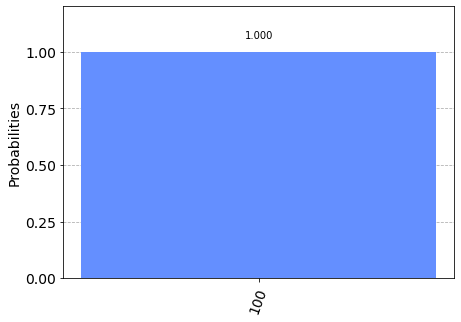
\includegraphics[width=0.7\linewidth]{./images/5qubit_sim.png}
	\caption{\textbf{Histogram:} 5 Qubit circuit executed on a simulator}%
	\label{fig:5qubit_sim}%
\end{figure}


\subsubsection{Executing the Quantum Circuit on an actual Quantum Computer}
\label{code:executing_the_quantum_circuit_on_a_quantum_computer}
\textbf{Importing the relevant libraries}
\label{code:importing_the_libraries_2}
\begin{lstlisting}[language=Python]
from qiskit.providers.ibmq import least_busy
from qiskit.tools.monitor import job_monitor
from qiskit.providers.ibmq.ibmqbackend import IBMQSimulator
# IBMQ.load_account(<API_Token>)
IBMQ.load_account()\end{lstlisting}
{\fontfamily{pcr}\selectfont <AccountProvider for IBMQ(hub='ibm-q', group='open',\par
project='main')>}
\vspace{3mm}

\textbf{Choosing the least busy backend}

\begin{lstlisting}[language=Python]
provider = IBMQ.get_provider('ibm-q')
q_comp = least_busy(
	[x for x in provider.backends() if not isinstance(x, IBMQSimulator)]
	)\end{lstlisting}
\vspace{3mm}

\textbf{Executing the circuit on a Quantum Computer}

\begin{lstlisting}[language=Python]
job = execute(circuit, q_comp, shots = 16384)
job_monitor(job)
print("results:", job.result().get_counts(circuit))
plot_histogram(job.result().get_counts(circuit))\end{lstlisting}

{\fontfamily{pcr}\selectfont
\noindent Job Status: job has successfully run

\noindent results:\par
\{`000': 819,\par
`001': 438,\par
`010': 157,\par
`011': 112,\par
`100': 12416,\par
`101': 1399,\par
`110': 877,\par
`111': 166\}}

\begin{figure}[h]%
	\centering
	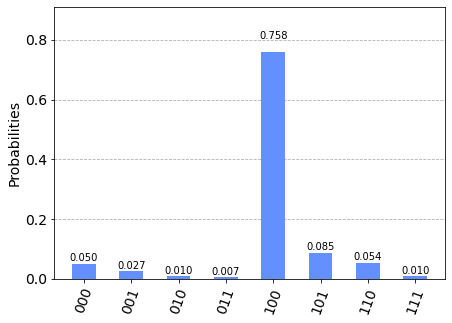
\includegraphics[width=0.9\linewidth]{./images/5qubit_act.png}
	\caption{\textbf{Histogram:} 5 Qubit circuit executed on an actual Quantum Computer}%
	\label{fig:5qubit_act}%
\end{figure}

	\subsection{Approach 2: 3 Cubit Solution}
	\label{solution:2}
		\textbf{Importing the libraries:}
This part is the same as \hyperref[code:importing_the_libraries]{`Importing the libraries'} section from the \hyperref[solution:1]{Approach 1}.

\textbf{Making the Quantum Circuit:}
\begin{lstlisting}[language=Python]
# Making the Qiskit Classes:
qreg_s1_to_m2 = QuantumRegister(1, 's1_to_m2')
qreg_s2_to_m1 = QuantumRegister(1, 's2_to_m1')
qreg_to_m3 = QuantumRegister(1, 'to_m3')
creg_measurements = ClassicalRegister(3, 'measurements')
circuit = QuantumCircuit(
	qreg_s1_to_m2,
	qreg_s2_to_m1,
	qreg_to_m3,
	creg_measurements
	)

# Initializing the Circuit:
ket_0 = [1, 0]
ket_1 = [0, 1]
quantumRead = [ket_1, ket_0]   # |10>
circuit.initialize(quantumRead[0], [qreg_s1_to_m2[0]])
circuit.initialize(quantumRead[1], [qreg_s2_to_m1[0]])

# Designing the circuit
circuit.ccx(qreg_s1_to_m2[0],qreg_s2_to_m1[0],qreg_to_m3[0])
circuit.x(qreg_s1_to_m2[0])
circuit.x(qreg_s2_to_m1[0])
circuit.barrier()
circuit.measure(qreg_to_m3[0], creg_measurements[0])
circuit.measure(qreg_s1_to_m2[0], creg_measurements[1])
circuit.measure(qreg_s2_to_m1[0], creg_measurements[2])
circuit.draw(output = 'mpl')\end{lstlisting}

\begin{figure}[h]%
	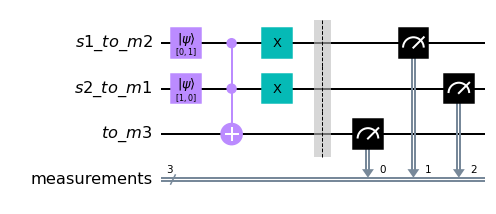
\includegraphics[width=0.85\linewidth]{./images/3qubit_qc.png}
	\caption{Circuit of the 3 Qubit Design}%
	\label{fig:3qubit_qc}%
\end{figure}

\textbf{Executing the circuits in both simulators and actual quantum computers:}
The codes are same as \hyperref[code:executing_the_quantum_circuit_on_a_simulator]{`Executing the Quantum Circuit on a Simulator'} and \hyperref[code:executing_the_quantum_circuit_on_a_quantum_computer]{`Executing the Quantum Circuit on an actual Quantum Computer'} section from the \hyperref[solution:1]{Approach 1}.

The result on the classical computer was exactly the same as the \hyperref[fig:5qubit_act]{previous result}. That on the Quantum Computer came out to be like \hyperref[fig:3qubit_act]{Figure 8}.

\begin{figure}[h]%
	\centering
	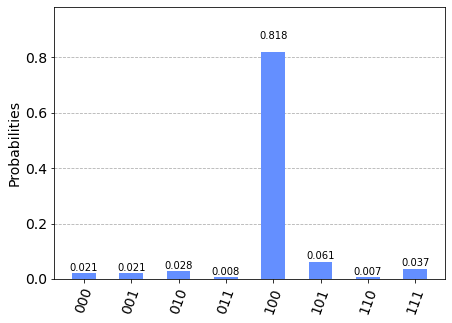
\includegraphics[width=0.85\linewidth]{./images/3qubit_act.png}
	\caption{\textbf{Histogram:} 3 Qubit Circuit executed on an actual Quantum Computer}%
	\label{fig:3qubit_act}%
\end{figure}  % solution
	
	
	
	
	
	
	
	
	% include the bibliographic references
	\pagebreak
	% \addcontentsline{toc}{section}{References}
	\bibliographystyle{apalike}
	\bibliography{mybib.bib}
	\nocite{*}

	% including the list of figures and the list of tables
	\listoffigures
	\listoftables

\end{document}